\section*{2.1 Método de bisección}

En esta sección consideraremos uno de los problemas más básicos del aproximación numérica, el \textbf{problema de encontrar una raíz}. Este proceso involucra encontrar una \textbf{raíz}, o solución, a una ecuación de la forma $f(x)=0$, para la función dada $f$. Una raíz de dicha ecuación también es llamada un \textbf{cero} de la función $f$.
\\

La primera técnica basada en el \textit{Teorema de valor intermedio}, es llamada \textbf{método de bisección} o \textbf{método de búsqueda binaria}.

Suponga $f$ una función continua definida en el intervalo $[a,b]$, con $f(a)$ y $f(b)$ de signos contrarios. El Teorema de valor intermedio implica la existencia de un número $p$ en $(a,b)$ tal que $f(p)=0$. Aunque el procedimiento funcionará si hay más de una raíz en el intervalo $(a,b)$, asumiremos que la raíz en este intervalo es única. El método requiere una repetida partición por la mitad (o bisección) de subintervalos de $[a,b]$, y, en cada paso, localizar la mitad que contiene a $p$.

\ Sea $a_1=a$, $b_1=b$ y dejemos que $p_1$ sea el punto medio de $[a,b]$; entonces

\begin{equation*}
    p_1=a_1+\frac{b_1-a_1}{2}=\frac{a_1+b_1}{2},
\end{equation*}

\begin{itemize}
    \item Si $f(p_1)=0$, entonces $p=p_1$ y hemos acabado.
    \item Si $f(p_1)\neq0$, entonces $f(p_1)$ tiene el mismo signo que $f(a_1)$ o $f(b_1)$.
    \begin{itemize}
        \item  Si $f(p_1)$ y $f(a_1)$ tienen el mismo signo, $p\in(p_1,b_1)$. Sea $a_2=p_1$ y $b_2=b_1$
        \item  Si $f(p_1)$ y $f(a_1)$ tienen signo opuesto, $p\in(a_1,p_1)$. Sea $a_2=a_1$ y $b_2=p_1$
    \end{itemize}
\end{itemize}

Entonces aplicar de nuevo el proceso al intervalo $[a_2,b_2]$. Esto produce el método descrito en el siguiente algoritmo con su respectiva representación geométrica.

\begin{tcolorbox}[colback=blue!15!]
\subsubsection*{Bisección}
Para encontrar la solución a $f(x)=0$ dada una función continua en el intervalo $[a,b]$, donde $f(a)$ y $f(b)$ tienen el signo opuesto:
\\ \\
ENTRADA Puntos límites $a$, $b$; tolerancia \textit{TOL}; número máximo de iteraciones $N_0$.

SALIDA La solución aproximada \textit{p} o mensaje de falla.

PASO 1 Asigna i=1;

\ \ \ \ \ \ \ \ \ \ \ \ \ \ \ \ \ \ \ \ \ \ $FA=f(a)$

PASO 2 Mientras $i\leq N_0$ ejecuta los pasos 3-6.

\ \ \ \  PASO 3 Asigna $p=a+(b-a)/2$; (calcula $p_i$)

\ \ \ \ \ \ \ \ \ \ \ \ \ \ \ \ \ \ \ \ \ \ \ \ \ $FP=f(p)$
    
\ \ \ \   PASO 4 Si $FP=0$ o $(b-a)/2<TOL$ entonces

\ \ \ \ \ \ \ \ \ \ \ \ \ \ \ \ \ \ SALIDA (p); (proceso completado exitosamente)

\ \ \ \ \ \ \ \ \ \ \ \ \ \ \ \ \ \ ALTO.

\ \ \ \   PASO 5 Asigna $i=i+1$
    
\ \ \ \   PASO 6 Si $FA\cdot FP>0$ entonces asigna $a=p$; (calcula $a_i,b_i$)

\ \ \ \ \ \ \ \ \ \ \ \ \ \ \ \ \ \ \ \ \ \ \ \ \ \ \ \ \ \ \ \ \ \ \ \ \ \ \ \ \ \ \ \ \ \ \ \ \ \ \ \ \ \ \ $FA=FP$

\ \ \ \ \ \ \ \ \ \ \ \ \ \ \ \ \ \ \ \ \ \ \ De otro modo asigna $b=p$ (FA no sufre cambios)

PASO 7 SALIDA ('El método falló después de $N_0$ iteraciones $N_0=$',$N_0$);

\ \ \ \ \ \ \ \ \ \ \ \ \ (El proceso fue exitoso.)

\ \ \ \ \ \ \ \ \ \ \ \ \ ALTO.


\end{tcolorbox}

\begin{figure*}[!h]
 \begin{center}
    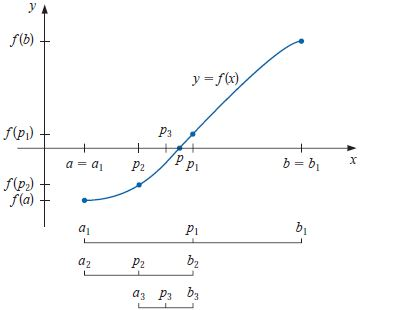
\includegraphics[width=0.8\textwidth]{Biseccion.JPG}
    %\caption{Rapidez de corte vs esfuerzo cortante MAB}
 \end{center}
\end{figure*} 

\subsubsection*{Ejemplo}
Muestra que $f(x)=x^3+4x^2-10=0$ tiene una raíz en $[1,2]$, y usa el método de bisección para determinar una aproximación a la raíz que tenga una precisión de al menos $10^{-4}$.

\textbf{Solución}. Dado que $f(1)=-5$ y $f(2)=14$ el teorema de valor intermedio asegura que ésta función, al ser continua, tiene una raíz en $[1,2]$.

Para la primera iteración del método de bisección usamos el punto medio de $[1,2]$ y obtenemos $f(1.5)=2.375>0$. Eso nos indica que debemos seleccionar el intervalo $[1,1.5]$ para la segunda iteración. Ahora encontramos que $f(1.25)=-796875>0$ entonces nuestro nuevo intervalo es $[1.25,1.5]$ con punto medio en $1.375$. Continuando de esta manera obtenemos la \ref{tab:tabla2}:

\begin{table}[h!]
\centering
    \begin{tabular}{||c c c c c||}
    \hline 
    \hline
        n & $a_n$ & $b_n$ & $p_n$ & $f(p_n)$ \\
    \hline 
    \hline 
        1 & 1.0 & 2.0 & 1.5 & 2.375 \\
        2 & 1.0 & 1.5 & 1.25 & -1.79687 \\
        3 & 1.25 & 1.5 & 1.375 & 0.16211 \\
        4 & 1.25 & 1.375 & 1.3125 & −0.84839 \\
        5 & 1.3125 & 1.375 & 1.34375 & −0.35098 \\
        6 & 1.34375 & 1.375 & 1.359375 & −0.09641 \\
        7 & 1.359375 & 1.375 & 1.3671875 & 0.03236 \\
        8 & 1.359375 & 1.3671875 & 1.36328125 & −0.03215 \\
        9 & 1.36328125 & 1.3671875 & 1.365234375 & 0.000072 \\
        10 & 1.36328125 & 1.365234375 & 1.364257813 & −0.01605 \\
        11 & 1.364257813 & 1.365234375 & 1.364746094 & −0.00799 \\
        12 & 1.364746094 & 1.365234375 & 1.364990235 & −0.00396 \\
        13 & 1.364990235 & 1.365234375 & 1.365112305 & −0.00194 \\
        \hline
        \hline 
    \end{tabular}
    \caption{Bisección}
    \label{tab:tabla2}
\end{table}



Como observación final, para determinar que subintervalo $[a_n.b_n]$ contiene la raíz de $f$, es mejor hacer uso de la función \textbf{signo}, que es definida como:

\begin{equation*}
    sgn(x)= \left\{ \begin{array}{lcc}
             -1 &   si  & x < 0 \\
             \\ 0 &  si &  x = 0 \\
             \\ 1 &  si  & x > 0
             \end{array}
   \right.
\end{equation*}

Dado que la prueba

\begin{equation*}
    sgn(f(a_n))sgn(f(p_n))<0 \ \ \ \ en \ vez \ de \  f(a_n)f(p_n)<0
\end{equation*}

da el mismo resultado pero evita la posibilidad de saturación o sub-desbordamiento en la multiplicación de $f(a_n)$ con $f(p_n)$